% ******************************************************** %
%              TEMPLATE DE INFORME ORGA2 v0.1              %
% ******************************************************** %
% ******************************************************** %
%                                                          %
% ALGUNOS PAQUETES REQUERIDOS (EN UBUNTU):                 %
% ========================================
%                                                          %
% texlive-latex-base                                       %
% texlive-latex-recommended                                %
% texlive-fonts-recommended                                %
% texlive-latex-extra?                                     %
% texlive-lang-spanish (en ubuntu 13.10)                   %
% ******************************************************** %


\documentclass[a4paper,]{article}
\usepackage[spanish]{babel}
\usepackage[utf8]{inputenc}
\usepackage{charter}   % tipografia
\usepackage{graphicx}
\usepackage[table,xcdraw]{xcolor}
%\usepackage{makeidx}
\usepackage{paralist} %itemize inline

\usepackage{float}
\usepackage{amsmath, amsthm, amssymb}
\usepackage{amsfonts}
%\usepackage{sectsty}
%\usepackage{charter}
%\usepackage{wrapfig}
\usepackage{listingsutf8}

% \setcounter{secnumdepth}{2}
\usepackage{underscore}
\usepackage{caratula}
\usepackage{url}
%\usepackage[superscript,biblabel]{cite}
%\usepackage{dibujitos}

\usepackage{amssymb}


\graphicspath{ {img/} {../graph/} }

% ********************************************************* %
% ~~~~~~~~              Code snippets             ~~~~~~~~~ %
% ********************************************************* %

\usepackage{color} % para snipets de codigo coloreados
\usepackage{fancybox}  % para el sbox de los snipets de codigo

\definecolor{litegrey}{gray}{0.94}

\newenvironment{codesnippet}{%
	\begin{Sbox}\begin{minipage}{\textwidth}\sffamily\small}%
	{\end{minipage}\end{Sbox}%
		\begin{center}%
		\vspace{-0.4cm}\colorbox{litegrey}{\TheSbox}\end{center}\vspace{0.3cm}}

\definecolor{mygreen}{rgb}{0,0.6,0}
\definecolor{mygray}{rgb}{0.5,0.5,0.5}
\definecolor{mymauve}{rgb}{0.58,0,0.82}

\lstset{ %
  backgroundcolor=\color{litegrey},
  basicstyle=\footnotesize,
  breakatwhitespace=true,
  breaklines=true,
  captionpos=b,                    % sets the caption-position to bottom
  mathescape=true,
  keepspaces=true,
  language=Python,
  showspaces=false,
  tabsize=2,                       % sets default tabsize to 2 spaces
  inputencoding=utf8/latin1
}

\newcommand{\cuidado}{{\large $\Delta$!!!} \hspace*{1em}}

\newcommand*{\QEDA}{\hfill\ensuremath{\blacksquare}}%
\newcommand*{\QEDB}{\hfill\ensuremath{\square}}%

% ********************************************************* %
% ~~~~~~~~         Formato de las páginas         ~~~~~~~~~ %
% ********************************************************* %

\usepackage{fancyhdr}
\pagestyle{fancy}

\renewcommand{\sectionmark}[1]{\markright{\thesection\ - #1}}

\fancyhf{}

\fancyhead[LO]{Sección \rightmark} % \thesection\
\fancyfoot[LO]{\small{Agustín Borgna, Cristian Vazquez, Gian Franco Lancioni, Juan Gonzalez Benitez - \textbf{Redes (TP1)}}}
\fancyfoot[RO]{\thepage}
\renewcommand{\headrulewidth}{0.5pt}
\renewcommand{\footrulewidth}{0.5pt}
\setlength{\hoffset}{-0.8in}
\setlength{\textwidth}{16cm}
%\setlength{\hoffset}{-1.1cm}
%\setlength{\textwidth}{16cm}
\setlength{\headsep}{0.5cm}
\setlength{\textheight}{25cm}
\setlength{\voffset}{-0.7in}
\setlength{\headwidth}{\textwidth}
\setlength{\headheight}{13.1pt}

\renewcommand{\baselinestretch}{1.1}  % line spacing

% ******************************************************** %


\begin{document}


\thispagestyle{empty}
\materia{Teoría de las Comunicaciones}
\submateria{Primer Cuatrimestre de 2017}
\titulo{Trabajo Práctico 1}
\subtitulo{ARP Sniffing}
\integrante{Borgna, Agustín}{079/15}{aborgna@dc.uba.ar}
\integrante{Gonzalez Benitez, Juan}{324/14}{gonzalezjuan.ab@gmail.com}
\integrante{Lancioni, Gian Franco}{234/15}{gianflancioni@gmail.com}
\integrante{Vazquez, Cristian}{056/10}{(cristianvazquez4@gmail.com}

\maketitle
\newpage

\thispagestyle{empty}
\vfill

\thispagestyle{empty}
\vspace{2cm}
\tableofcontents
\newpage


\normalsize
\newpage
\twocolumn
A modo muy general, con el objetivo de analizar distintas redes locales, vamos a modelar ciertos comportamientos en el tráfico como fuentes de Teoría de la Información y poder extraer conclusiones concretas partiendo de las herramientas conocidas, particularmente los conceptos de entropía de la fuente e información de un símbolo en dicha fuente, para estudiar dichas fuentes.
\section{Introducción}
\subsection{ARP}
En particular nos interesa analizar las interacciones que se dan entre hosts de la red con el fin resolver direcciones de capa de red hacia capa de enlace, usualmente IP a MAC. Estas interacciones son propias del \emph{ARP (protocolo de resolución de direcciones)} \footnote{https://en.wikipedia.org/wiki/Address_Resolution_Protocol}, el cual cumple un rol crucial en lo que conocemos como \emph{internetworking}.

Se trata de un protocolo de \emph{request} y \emph{response}, implementados a partir de paquetes \emph{'who-has'}, que preguntan a un dominio de broadcast por la \emph{MAC address} de una IP particular, y paquetes \emph{'is-at'} que responden de manera unicast al emisor del paquete 'who-has'.

El tipo del paquete se determina por el campo de operación de dicho paquete, del cual haremos amplio uso.

Por supuesto, dicho protocolo no se ejecuta cada vez que se quiera efectuar una transmisión, sino que los resultados se almacenan temporalmente una \emph{cache} para agilizar tiempos.

\subsection{Herramientas y resolución de primer etapa}
Cada una de las capturas de red que hicimos (una por cada integrante del grupo), se hizo con el programa \emph{TShark}, versión \emph{terminal-based} del packet sniffer \emph{Wireshark}.

Los paquetes obtenidos los manipulamos con el framework \emph{Scapy} de \emph{Python} que nos permite acceder a los campos de cada uno y, por ejemplo, determinar si tiene capa \emph{ARP} y (de ser así) su destino buscado.

\subsubsection{Primer ejercicio}

Lo primero que se nos pide es modelar cada red como una fuete de información binaria $S$ de memoria nula con símbolos en $\{S_{unicast},\ S_{broadcast}\}$.

Para implementar la fuente simplemente contaremos la cantidad de paquetes $p$ tales que $p.dst =$ 'ff:ff:ff:ff:ff:ff' (i.e la dirección MAC de destino de broadcast). Dicha implementación está en \emph{entro.py} y se encarga de imprimir por pantalla la entropía de la fuente y las ocurrencias de cada símbolo para una secuencia dada de paquetes.

Por lo tanto dicha fuente se abstrae de la identidad de los nodos de la red y los trata indiscriminadamente como emisores de símbolos según la dirección de capa de enlace de sus paquetes.

A modo analítico, la fuente $S$ de cada red permite entender de qué manera se comunican los hosts de la red.

Por ejemplo, al tratarse de conexiones predominantemente dirigidas, resultaría extraño que los paquetes de broadcast fueran mayoría en el tráfico de la red. Y en caso contrario, la fuente haría visibles escenarios particulares de topologías o comunicaciones entre hosts.

\subsubsection{Segundo ejercicio}

El segundo ejercicio consistió en modelar una nueva fuente de información $S_1$ de memoria nula, con el objetivo de distinguir, en lugar de tipos de destinos como lo hacía $S$, los propios nodos (hosts) de la red.

Dicha distinción se hizo a partir de los paquetes \emph{ARP}, y la implementación se encuentra en \emph{distinguidos.py}.

Lo que hicimos fue considerar como símbolos las \emph{IPs} de request de los mensajes 'who-has'. De esta manera, los símbolos con menos información son aquellos más solicitados.

Entonces los nodos distinguidos, con la finalidad de exponer aquellos más 'importantes' en la red, los consideramos como aquellos símbolos $s$ tales que $I(s) < H(S_1)$ siendo $I(s)$ la información del nodo s en la fuente $S_1$ y $H(S_1)$ la entropía de la fuente.

Siguiendo con esta idea, es de esperarse que los nodos más solicitados, como los \emph{default gateways} aparezcan siempre entre los distinguidos.

\newpage
\onecolumn
\section{Mediciones realizadas}
Ahora mostraremos los datos obtenidos en todas las mediciones, considerando las herramientas obtenidas en los dos ejercicios de la primera etapa mas un conjunto de gráficos que aporten nuevos datos para poder analizar.

\subsection{Red 'Tatooine-lan'}
Esta medición se trata de una red Wi-Fi doméstica de 4 dispositivos activos con un tiempo de escucha de 20 minutos. Dos de las máquinas estaban usando servicios de streaming de video.
\\

Mientras se realizaba la medición también se borraron los registros (comando 'arp -d $<host\_ip>$' en linux) la caché ARP en el dispositivo cuya IP pública es 190.168.0.14 y privada 192.168.0.12 con el objetivo de forzar un handshake en dicho protocolo con el default gateway de la red.
\\

Además, se reinició un dispositivo mientras se corría la escucha.

\subsubsection{Fuente S}
En la medición se contaron entre todos los paquetes del archivo \emph{.pcap} con la herramienta el ejercicio 1:

        \begin{itemize}
            \item 69834 paquetes unicast
            \item 289 paquetes broadcast (p.dst = 'ff:ff:ff:ff:ff')
            \item 70123 paquetes en total
        \end{itemize}

Dejando una entropía $H(S) = 0.03858550573957047$ y la siguiente distribución en la información de los símbolos $S_{broadcast}$ y $S_{unicast}$:

\begin{figure}[H]
	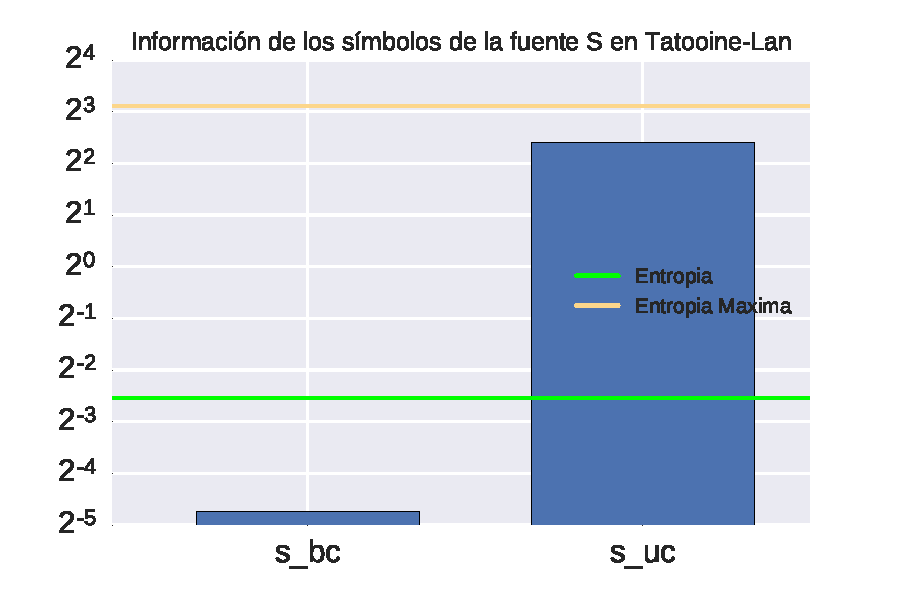
\includegraphics[width=15cm, height=12cm, keepaspectratio]{../img/barras-Tatooine-Lan.pdf}
\end{figure}

\newpage
\subsubsection{Grafo de conectividad de la red}
Con el fin de analizar de mejor manera la topología de la red también armamos un grafo entre los nodos de la red que muestre el tráfico de paquetes ARP sensado. Cada nodo está asociado a una IP y un eje entre una $IP_1$ y $IP_2$ significa que se sensó un paquete \emph{'who-has'} emitido por $IP_1$ consultando por la dirección MAC de $IP_2$.

\begin{figure}[H]
	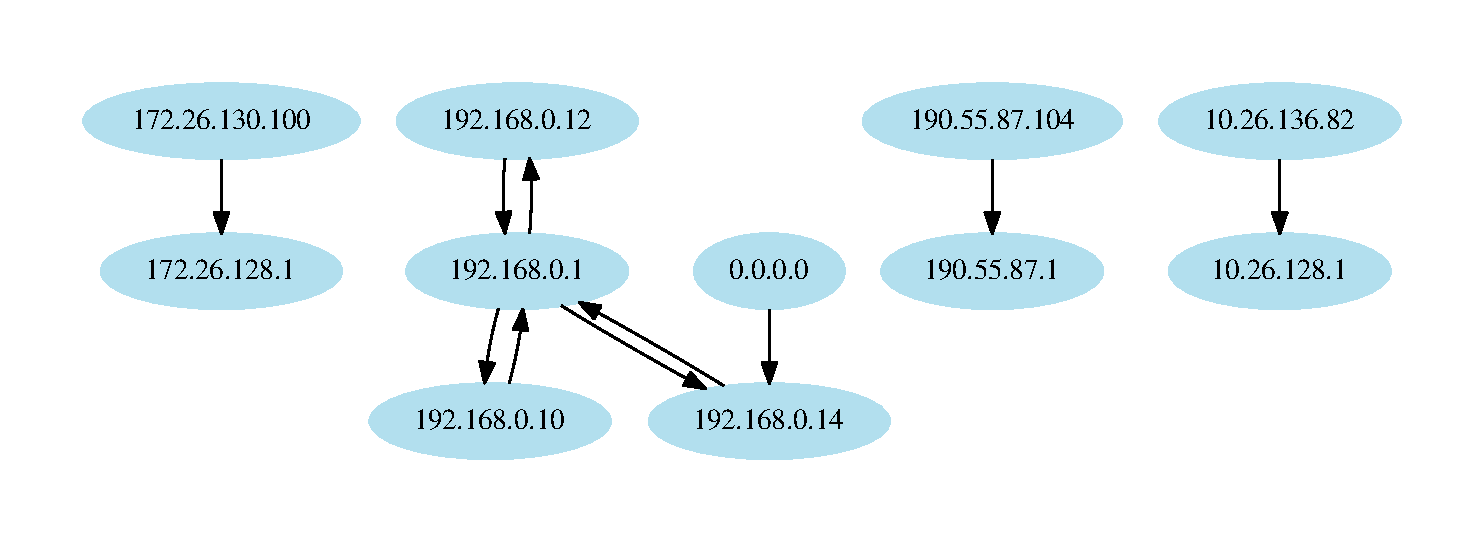
\includegraphics[width=15cm, height=8.7cm]{../img/red-Tatooine-Lan.pdf}
\end{figure}

Se puede notar que ninguno de los otros dispositivos mecionados, al margen de aquel para el cual flusheamos la caché ARP, hizo un request de tipo \emph{'who-has'} durante el sniff usando su IP pública. Dicho comportamiento se repite en las otras redes aledañas en las cuales un único nodo envía un paquete \emph{'who-has'} a una IP con el último octeto en 1 (candidatos a routers).
\\

Pero, por otro lado, se puede ver buena actividad en una red que parece corresponderse con el rango 192.168.0.0/16 reservado para IPs privadas. Como la capa de enlace se encarga de que las redes privadas no se solapen, podemos afirmar que se trata de la red a la que nos conectamos durante la medición.
\\

Es interesante la aparición de una IP 0.0.0.0, la cual se asigna a dispositivos en diferentes situaciones. Entre ellos, cuando un dispositivo se inicializa en una red y envía su primer paquete DHCP (sin conocer todavía su IP en la red). Por lo tanto, tiene sentido que dicha interacción se deba al dispositivo reiniciado mencionado antes.

\subsubsection{Información y nodos distinguidos}
Haciendo uso de la herramienta del ejercicio 2 para distinguir nodos de la red respecto de sus respectivos símbolos en la fuente $S_1$ en caso de que aporten menor información que la entropía de dicha fuente, encontramos únicamente al nodo 192.168.0.1 como nodo distinguido.
\\

Las direcciones con los dos últimos octetos en 0.1 en redes 192.168.0.0/16 son comunes para IPs de interfaces de routers. Lo que significaría que nuestro código fue capaz de encontrar al menos un default gateway, particularmente por el que más nodos consultaron.

\begin{figure}[H]
	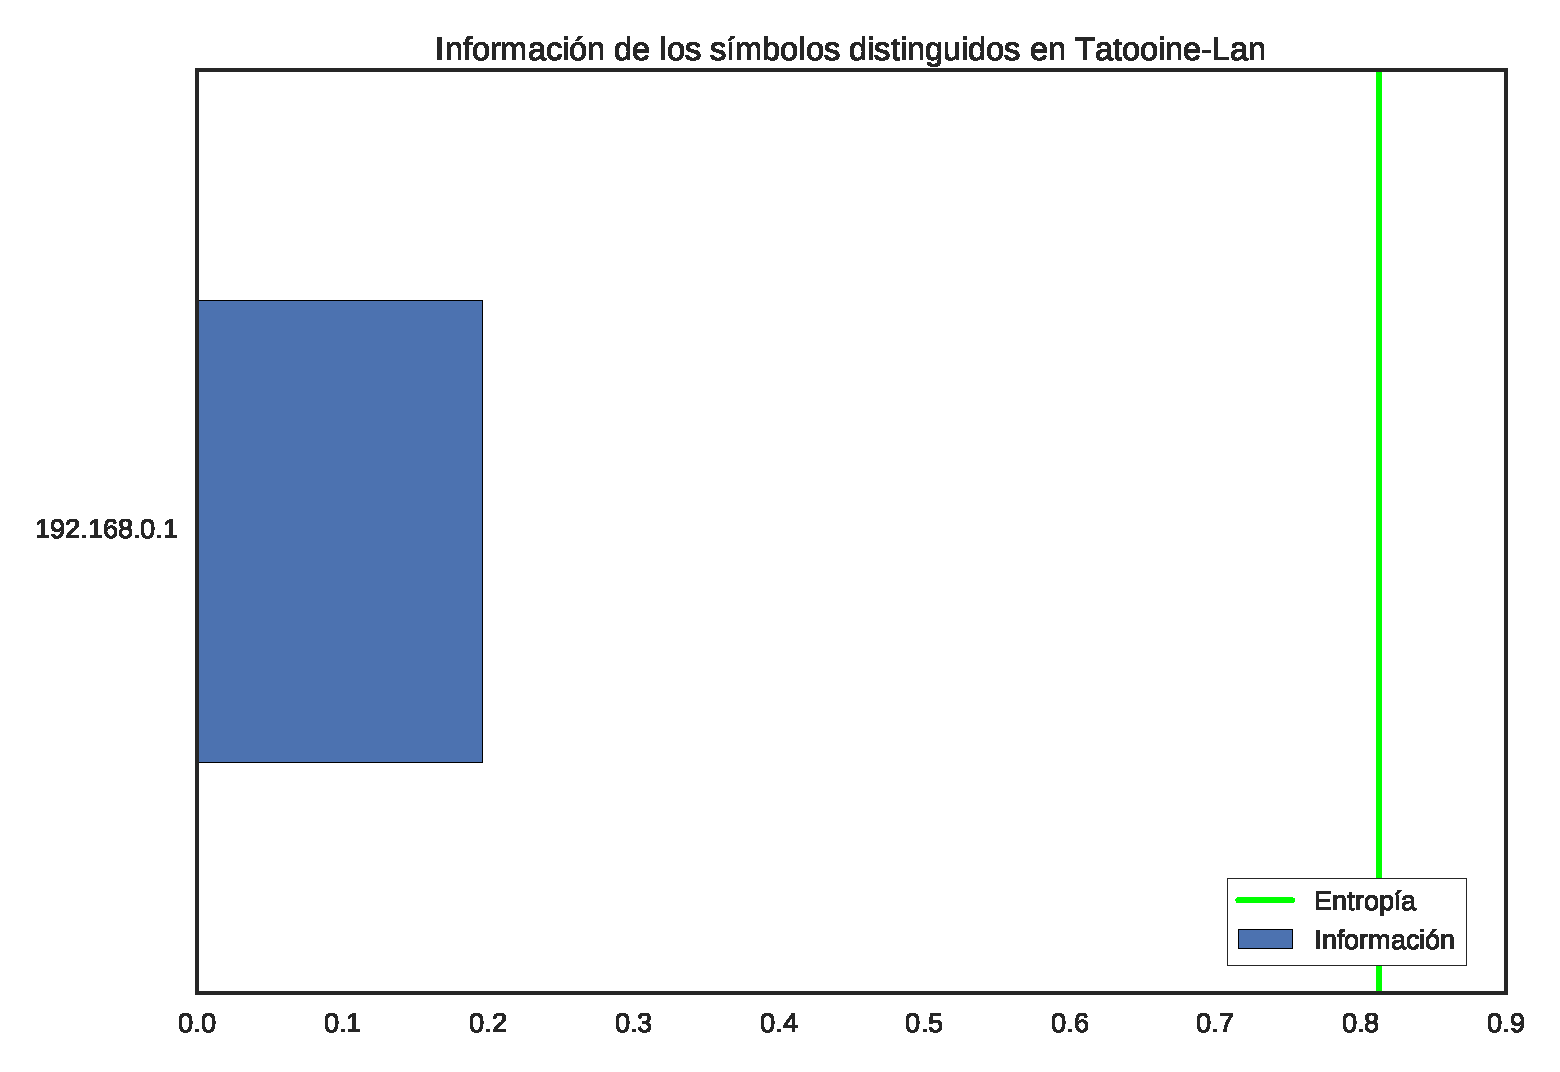
\includegraphics[width=15cm, height=8cm]{../img/distinguidos-Tatooine-Lan.pdf}
\end{figure}

\newpage
\appendix

%\newpage
%\bibliography{bibliography}{}
%\bibliographystyle{plain}

\end{document}
